\section{Training labels, cost and latency}
\label{sec:comparison}

A zero-shot model is paid per prediction and needs no labels; a supervised one needs labels and a
training run and then predicts almost for free. Figure~\ref{fig:f1labels} puts the four models
on one axis and Table~\ref{tab:costs} adds what each costs and how long a prediction takes. Every
cost is computed from recorded quantities: Jev's token counts at its published price, and the
billable seconds of each cloud job at the instance's list price.

\begin{figure}[t]
  \centering
  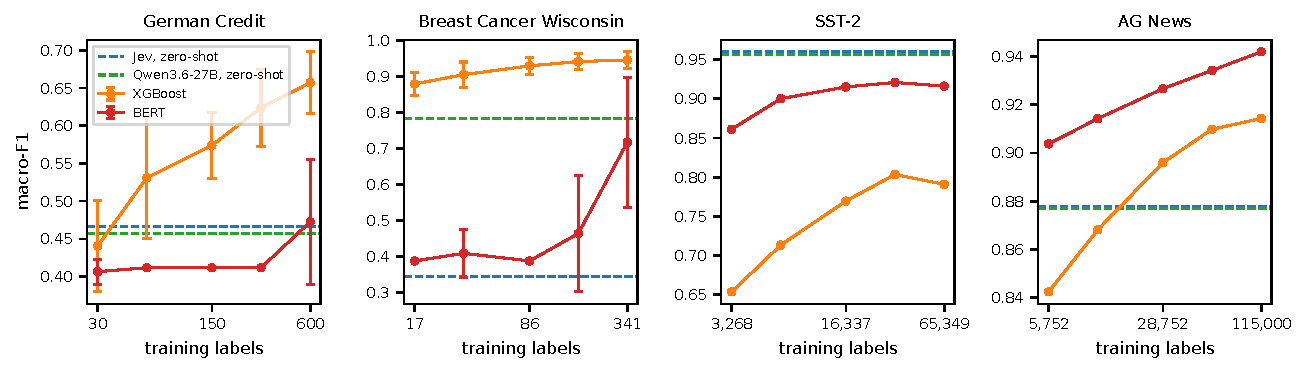
\includegraphics[width=\linewidth]{generated/figs/f1_by_labels}
  \caption{Macro-F1 on the evaluation examples against the number of training labels. Curves:
    supervised models. Dashed lines: zero-shot models, which use no training labels.}
  \label{fig:f1labels}
\end{figure}

\begin{table}[t]
  \caption{Labels, cost in USD and latency. Training cost is the whole recorded job, including
    model selection and the learning curve. Cost per 1,000 predictions: Jev, mean recorded
    request cost; Qwen, the billed scoring job allocated by scoring time, with inference time
    only in parentheses; XGBoost and BERT, measured batch inference time at list price. Latency:
    Jev, one API request; Qwen, one item sent alone, with batch throughput in parentheses;
    XGBoost and BERT, batch inference time per item.}
  \label{tab:costs}
  \centering\small
  \setlength{\tabcolsep}{4pt}
  \fittable{\begin{tabular}{llrcrll}
\toprule
Dataset & Model & Labels & Macro-F1 & Training & Per 1,000 & Latency \\
\midrule
\multirow{4}{*}{German Credit} & Jev & 0 & 0.467 & -- & 0.022 & 0.15\,s \\
 & Qwen3.6-27B & 0 & 0.457 & -- & 0.683 (0.642) & 0.95\,s (2.5/s) \\
 & XGBoost & 600 & 0.657 & 0.0097 & $<$0.0001 & 1.3\,$\mu$s \\
 & BERT & 600 & 0.473 & 0.148 & 0.0003 & 0.76\,ms \\
\addlinespace
\multirow{4}{*}{Breast Cancer Wisconsin} & Jev & 0 & 0.343 & -- & 0.030 & 0.14\,s \\
 & Qwen3.6-27B & 0 & 0.783 & -- & 1.34 (1.26) & 1.10\,s (1.3/s) \\
 & XGBoost & 341 & 0.945 & 0.010 & $<$0.0001 & 3.1\,$\mu$s \\
 & BERT & 341 & 0.716 & 0.129 & 0.0004 & 1.26\,ms \\
\addlinespace
\multirow{4}{*}{SST-2} & Jev & 0 & 0.960 & -- & 0.015 & 0.15\,s \\
 & Qwen3.6-27B & 0 & 0.956 & -- & 0.352 (0.331) & 0.92\,s (4.8/s) \\
 & XGBoost & 65{,}349 & 0.791 & 0.024 & $<$0.0001 & 0.01\,ms \\
 & BERT & 65{,}349 & 0.916 & 0.457 & $<$0.0001 & 0.19\,ms \\
\addlinespace
\multirow{4}{*}{AG News} & Jev & 0 & 0.878 & -- & 0.018 & 0.15\,s \\
 & Qwen3.6-27B & 0 & 0.877 & -- & 0.586 (0.551) & 0.93\,s (2.9/s) \\
 & XGBoost & 115{,}000 & 0.914 & 0.157 & $<$0.0001 & 0.06\,ms \\
 & BERT & 115{,}000 & 0.942 & 1.09 & 0.0001 & 0.31\,ms \\
\bottomrule
\end{tabular}
}
\end{table}

With enough labels a fine-tuned encoder overtakes both zero-shot models on topic classification:
BERT reaches macro-F1 \MacroFOneBertAgnews{} on AG News against \MacroFOneJevAgnews{} for Jev,
and first matches Jev at \LabelsToMatchJevBertAgnews{} training labels (XGBoost:
\LabelsToMatchJevXgbAgnews). On SST-2 neither supervised model matches the zero-shot ones at any
size tried: BERT reaches \MacroFOneBertSst{} with all \NTrainSst{} labels, against
\MacroFOneJevSst{} for Jev. On the tabular datasets XGBoost needs only its smallest training set
to exceed both zero-shot models.

A Jev prediction cost USD~\CostPerKJevSst{} to USD~\CostPerKJevWdbc{} per 1,000, depending on
prompt length, and took \JevLatencySst\,s. Self-hosting Qwen on \texttt{\QwenScoringInstance}
cost USD~\CostPerKQwenSst{} to USD~\CostPerKQwenWdbc{} per 1,000, which is \CostRatioQwenJevSst{}
to \CostRatioQwenJevWdbc{} times Jev's price, at \QwenLatencySst{} to \QwenLatencyWdbc\,s per
single item. The supervised models are cheaper per prediction by orders of magnitude once
trained; their cost is the training run (at most USD~\TrainUSDBertAgnews{} for BERT) and, above
all, the labels. Letting Qwen reason before answering raised its macro-F1 on every dataset on a
\ThinkSubsampleN-item sample (for example \ThinkSubFOneQwenWdbc{} to
\ThinkSubFOneQwenThinkWdbc{} on Breast Cancer Wisconsin) at many times the compute
(Table~\ref{tab:thinking}). Appendix~\ref{app:learning} gives the accuracy curves
(Figure~\ref{fig:learning}) and every point of both curves (Table~\ref{tab:learning}).
